\begin{frame}{Models as Approximations}
  \begin{columns}[c]
    \begin{column}{0.8\linewidth}
      \begin{itemize}
        \item Human minds and artificial systems never grasp reality directly; we use simplified representations called \bhighlight{models}.
        \item George E.P. Box famously stated: \\
              \emph{``All models are wrong, but some are useful.''}
        \item Our goal isn't perfect truth, but \bhighlight{useful approximations} that help us predict and interact with the world.
      \end{itemize}
    \end{column}
    \begin{column}{0.2\linewidth}
      \begin{figure}
        \centering
        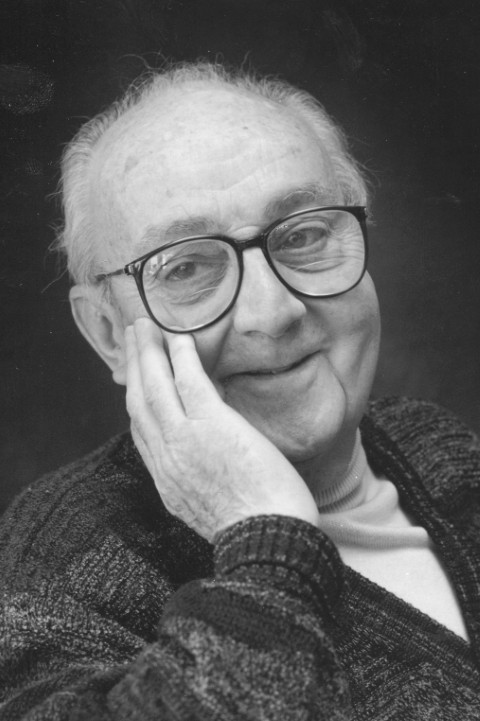
\includegraphics[width=\columnwidth]{images/george-ep-box.jpg}
        \caption{George E.P. Box --- One of the great statistians of the 20th century. \gcite{\href{https://commons.wikimedia.org/w/index.php?curid=115167166}{Source}}}
      \end{figure}
    \end{column}
  \end{columns}
\end{frame}

\begin{frame}{Observations and Reality}
  \begin{columns}[c]
    \begin{column}{0.6\linewidth}
      \begin{itemize}
        \item Our understanding comes from \bhighlight{observations}, which are samples or instances of reality.
        \item We assume there's an underlying \bhighlight{data-generating process} that creates the data we observe.
      \end{itemize}
    \end{column}
    %
    \begin{column}{0.4\linewidth}
      \begin{figure}
        \centering
        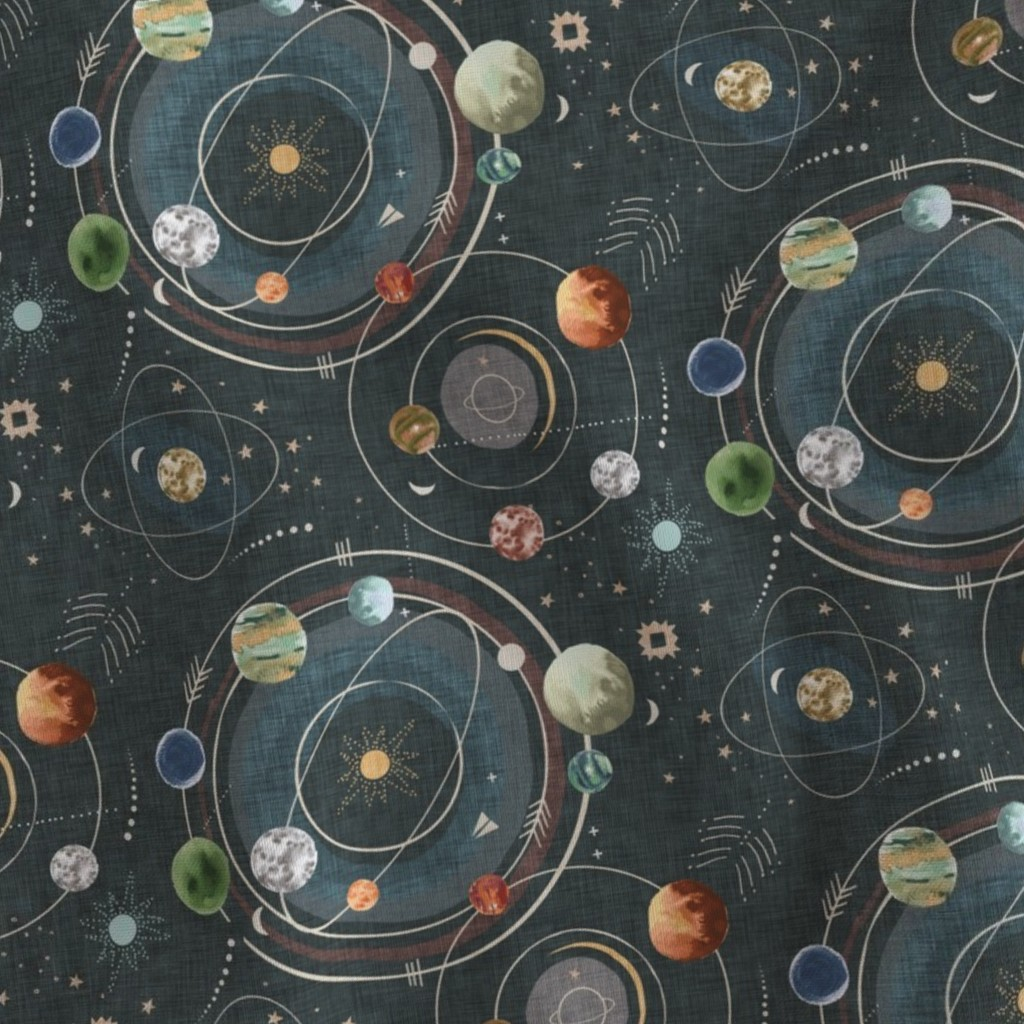
\includegraphics[width=\columnwidth]{images/universe.jpg}
        \caption{The data-generating process in our universe is the hidden ``source code'' that makes the laws of physics be the way they are. \gcite{\href{https://www.spoonflower.com/en/fabric/11122531-space-map-charcoal-med-by-nouveau_bohemian}{Source}}}
      \end{figure}
    \end{column}
  \end{columns}
\end{frame}

\begin{frame}{Observations and Reality}
  \begin{itemize}
    \item If our observations are good representations, we can learn rules and patterns that \bhighlight{generalize} to new situations.
    \item But how do we choose between multiple possible models?
  \end{itemize}
\end{frame}

\begin{frame}{Maximum Likelihood}
  \framesubtitle{Choosing the Best Model}
  \begin{itemize}
    \item A widely-used principle for selecting a model is \bhighlight{maximum likelihood}.
    \item Intuitively, it means choosing the model under which the observed data would have the \emph{highest probability} of occurring.
    \item Imagine flipping a coin:
          \begin{itemize}
            \item If you see heads 90 out of 100 times, which is more likely—a fair coin, or a biased one?
          \end{itemize}
    \item Maximum likelihood helps us quantify this intuition mathematically, guiding our choice of models based on observations.
  \end{itemize}
\end{frame}

% -------------------------------------------------------------------
\begin{frame}{Model Parameters}
  \framesubtitle{Defining a Hypothesis Space}
  \begin{itemize}
    \item A \bhighlight{model} is really a family of possible explanations for our data.
    \item We index each candidate by a vector of \bhighlight{parameters} $\theta\in\Theta$:
          \[
            p(x \mid \theta), \quad \theta = (\theta_1, \theta_2, \dots).
          \]
    \item Changing $\theta$ “moves” us to a different hypothesis about how data were generated.
    \item Learning = selecting the best $\theta$ given what we've actually observed.
  \end{itemize}
\end{frame}

\begin{frame}{Model Parameters}
  % \framesubtitle{...}
  \begin{figure}
    \centering
    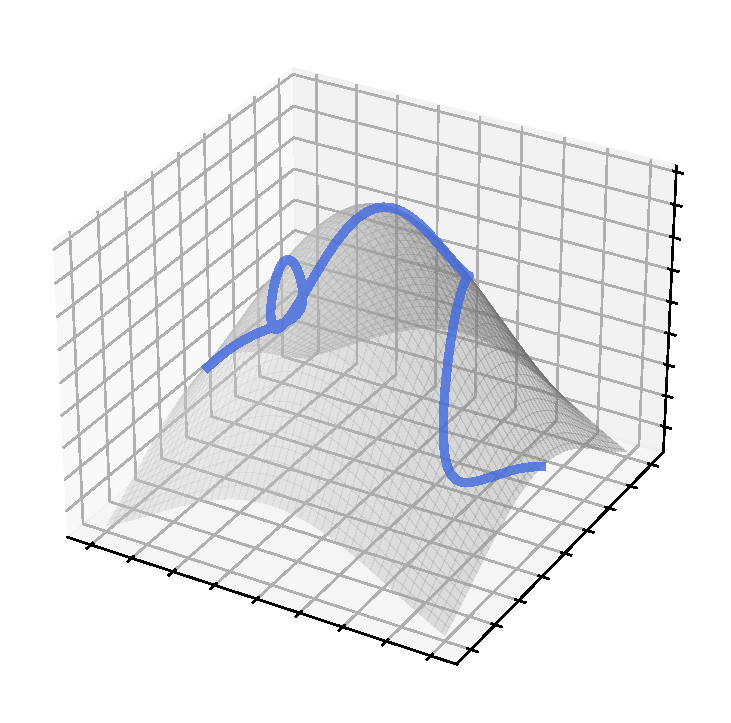
\includegraphics[height=0.65\textheight]{images/model_family_on_hypothesis_space.pdf}
    \caption{Visualization of a model family (red 2D curve) over a hypothesis space (transparent 3D curve).}
  \end{figure}
\end{frame}

% -------------------------------------------------------------------
\begin{frame}{The Likelihood Function}
  \framesubtitle{How Well Does $\theta$ Explain the Data?}
  \begin{itemize}
    \item Suppose our dataset is $D = \{x_1, x_2, \dots, x_N\}$.
    \item We quantify the \emph{fit} of parameters $\theta$ via the \bhighlight{likelihood}:
          \[
            L(\theta;D) \;=\;\prod_{i=1}^N p\bigl(x_i \mid \theta\bigr).
          \]
    \item Rather than “probability of $\theta$,” think of $L(\theta;D)$ as “how plausible is $\theta$ \emph{given} the observed data?”
    \item Larger $L(\theta)$ means the model under $\theta$ would have made our observations more likely.
  \end{itemize}
\end{frame}

\begin{frame}{The Likelihood Function}
  % \framesubtitle{...}
  \begin{figure}
    \centering
    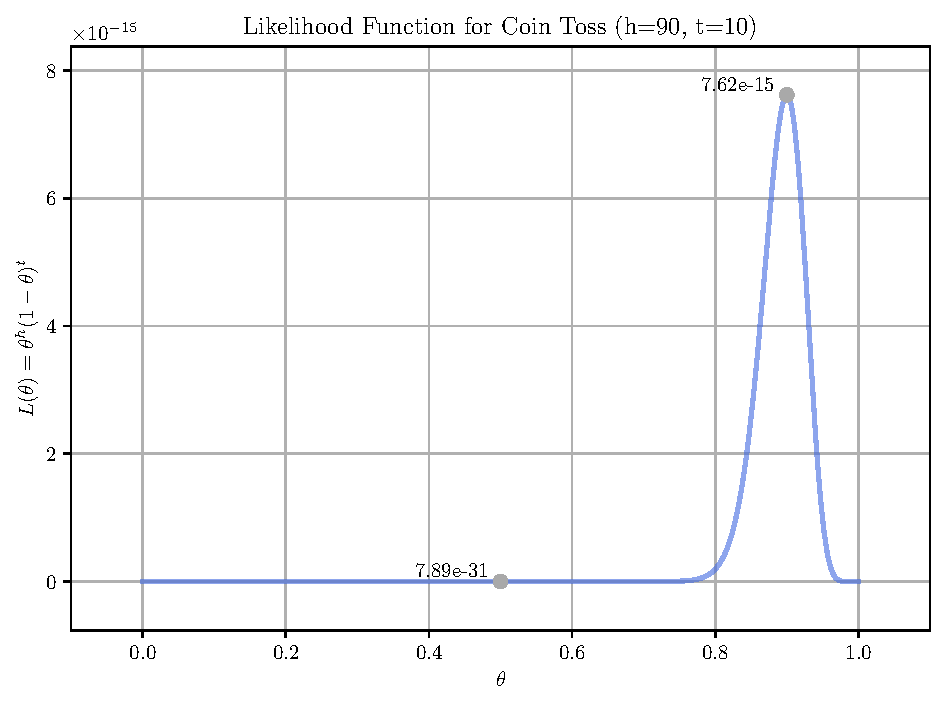
\includegraphics[height=0.65\textheight]{images/coin_toss_likelihood.pdf}
    \caption{Likelihood plot for a biased coin.}
  \end{figure}
\end{frame}

% -------------------------------------------------------------------
\begin{frame}{Log-Likelihood}
  \framesubtitle{Simplifying Optimization}
  \begin{itemize}
    \item Products can get unwieldy; take logs to turn products into sums:
          \[
            \ell(\theta;D) \;=\;\log L(\theta;D)
            \;=\;\sum_{i=1}^N \log p(x_i \mid \theta).
          \]
    \item $\ell(\theta)$ is called the \bhighlight{log-likelihood}.
    \item Maximizing $\ell(\theta)$ is equivalent to maximizing $L(\theta)$, but often easier to differentiate.
    \item In many cases we find a closed-form solution; otherwise we use \bhighlight{gradient-based} search which will be explored in later lectures.
  \end{itemize}
\end{frame}

\begin{frame}{Log-Likelihood}
  % \framesubtitle{...}
  \begin{figure}
    \centering
    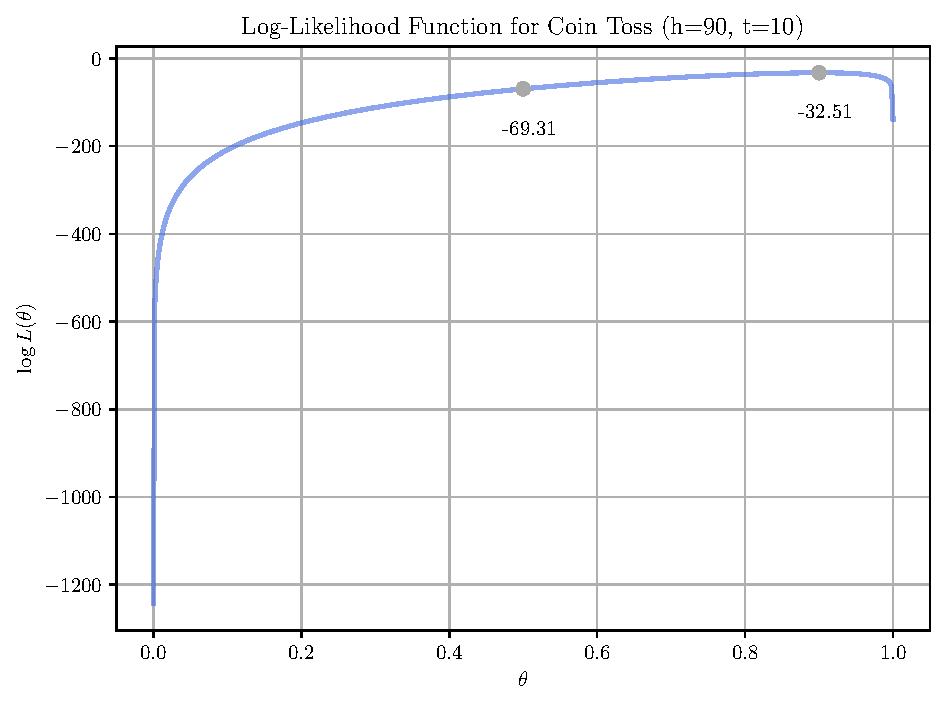
\includegraphics[height=0.65\textheight]{images/coin_toss_log_likelihood.pdf}
    \caption{Log-likelihood plot for the same biased coin as before.}
  \end{figure}
\end{frame}

% -------------------------------------------------------------------
\begin{frame}{Maximum Likelihood Estimation}
  \framesubtitle{Picking the Best Parameters}
  \begin{itemize}
    \item The core rule is
          \[
            \hat\theta_{\text{MLE}}
            \;=\;
            \argmax_{\theta\in\Theta}\;L(\theta;D)
            \;=\;
            \argmax_{\theta}\;\ell(\theta;D).
          \]
    \item This is our formal definition of “learning” in a statistical model:
          choose the hypothesis (parameters) under which the data are most probable.
  \end{itemize}
\end{frame}

% -------------------------------------------------------------------
{
\setframecolor{Crimson}
\begin{frame}{Coin Toss Pop Quiz}
  \framesubtitle{Estimating a Biased Coin}
  \begin{itemize}
    \item Each trial \(x_i\) is either heads (\(\mathrm{H}\)) or tails (\(\mathrm{T}\)); our model assumes \(\theta\) is the probability of heads.
    \item \textbf{Q1:} Write down the likelihood \(L(\theta)\) for observing \(h\) heads and \(t\) tails.
    \item \textbf{Q2:} Express the log-likelihood \(\ell(\theta)\).
    \item \textbf{Q3:} Compute the value of \(\theta\) that maximizes \(\ell(\theta)\).
  \end{itemize}
\end{frame}

\begin{frame}{Coin Toss Example — Solutions}
  \framesubtitle{Estimating a Biased Coin}
  \begin{itemize}
    \item \textbf{Likelihood:}
          \[
            L(\theta)
            = \theta^{\,h}\,(1-\theta)^{\,t}.
          \]
    \item \textbf{Log-likelihood:}
          \[
            \ell(\theta)
            = h\log\theta \;+\; t\log(1-\theta).
          \]
    \item \textbf{Maximizer:}
          \[
            \frac{d\ell}{d\theta}
            = \frac{h}{\theta} - \frac{t}{1-\theta} = 0
            \;\Longrightarrow\;
            \hat\theta = \frac{h}{h+t}.
          \]
    \item \emph{Intuition: “frequency = probability.”}
  \end{itemize}
\end{frame}
}

% -------------------------------------------------------------------
\begin{frame}{What Is a Random Variable?}
  \framesubtitle{From Real-World to Numbers}
  \begin{itemize}
    \item A \bhighlight{random variable} $X$ is just a way to turn an uncertain outcome into a number.
    \item Examples:
          \begin{itemize}
            \item Tossing a coin: $X=1$ for heads, $0$ for tails.
            \item Measuring temperature: $X$ = today's temperature in °C.
          \end{itemize}
    \item Each possible outcome has some \emph{chance} (probability) of happening.
  \end{itemize}
\end{frame}

% -------------------------------------------------------------------
\begin{frame}{The ``True'' Average (Expectation)}
  \framesubtitle{What We'd Get with Infinite Data}
  \begin{itemize}
    \item If we could repeat an experiment forever, the \bhighlight{expected value} (or \emph{population mean}) of $X$ is:
          \[
            \mu = \mathbb{E}[X] \;=\; \sum_x x\cdot P(X=x)
            \quad\bigl(\text{or } \int x\,p(x)\,dx\bigr).
          \]
    \item Informally: “where would the average settle if we could sample forever?”
    \item In practice, we don't know $\mu$ because we can't sample infinitely.
  \end{itemize}
\end{frame}

% -------------------------------------------------------------------
\begin{frame}{Sample Mean}
  \framesubtitle{What We Actually Observe}
  \begin{itemize}
    \item Suppose we collect $N$ measurements: $X_1, X_2, \dots, X_N$.
    \item Their \bhighlight{sample mean} is
          \[
            \overline{X} = \frac{1}{N}\sum_{i=1}^N X_i.
          \]
    \item This is the average we compute on our finite data.
    \item Question: \emph{How close} is $\overline{X}$ to the true mean $\mu$?
  \end{itemize}
\end{frame}

% -------------------------------------------------------------------
\begin{frame}{Law of Large Numbers}
  \framesubtitle{How ``quantity'' can improve ``quality''}
  \begin{itemize}
    \item The \bhighlight{Law of Large Numbers} says:
          \[
            \bar X \;\to\; \mu
            \quad\text{as}\quad N\to\infty.
          \]
    \item In plain terms: “With more data, the sample mean gets closer to the true mean.”
    \item This justifies using $\overline{X}$ as an estimate for $\mu$ when $N$ is large.
  \end{itemize}
\end{frame}

\begin{frame}{Law of Large Numbers}
  % \framesubtitle{...}
  \begin{figure}
    \centering
    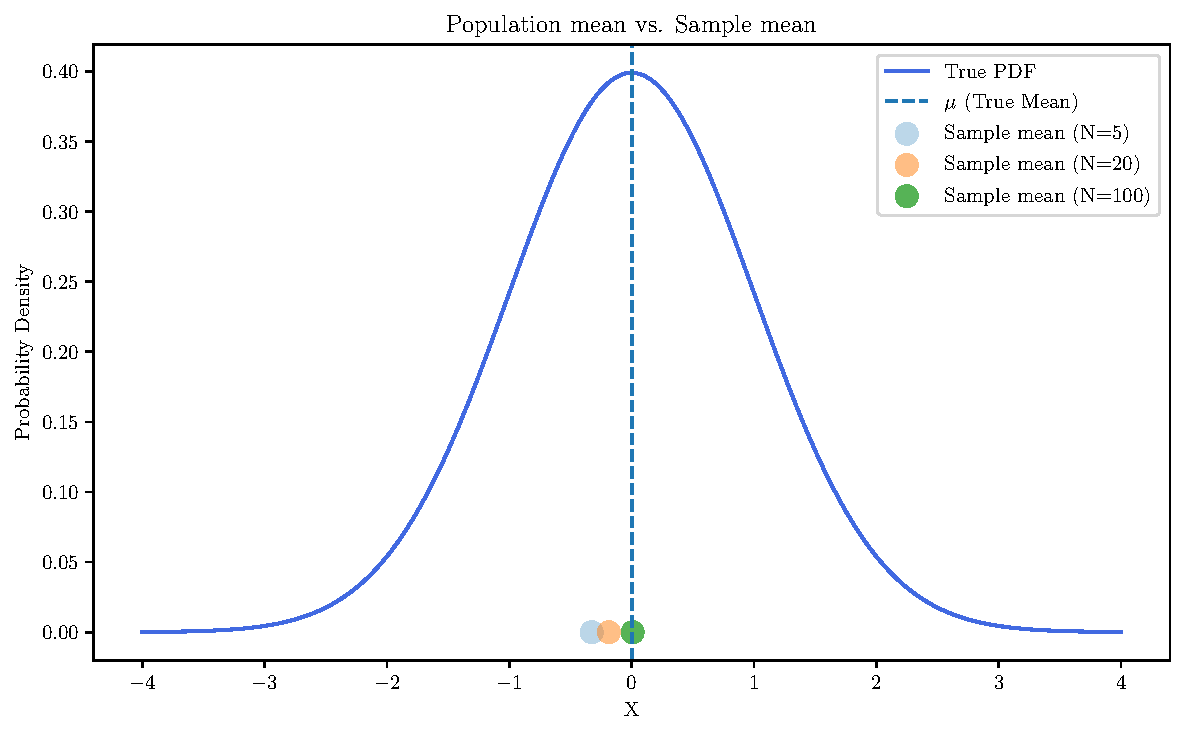
\includegraphics[height=0.65\textheight]{images/pop_mean_vs_sample_mean.pdf}
    \caption{Sample mean for three samples of the Normal distribution.}
  \end{figure}
\end{frame}

% -------------------------------------------------------------------
\begin{frame}{Measuring our mistakes}
  \framesubtitle{Loss functions}
  \begin{itemize}
    \item In learning we make predictions $f(x;\theta)$ and compare to true $y$.
    \item A \bhighlight{loss function} $\ell(y, f(x;\theta))$ assigns a \emph{numeric cost} to each mistake.
    \item Examples:
          \[
            \ell_{\text{0-1}} = \begin{cases}0 & \text{correct}\\1 & \text{wrong}\end{cases}
            ,\quad
            \ell_{\text{sq}}=(y - f(x))^2.
          \]
  \end{itemize}
\end{frame}

% -------------------------------------------------------------------
\begin{frame}{True Risk vs.\ Empirical Risk}
  \framesubtitle{Infinite Data vs.\ Finite Data}
  \begin{itemize}
    \item \bhighlight{True risk}:
          \[
            R(\theta)
            = \mathbb{E}\bigl[\ell(y, f(x;\theta))\bigr]
            \quad\text{(if we had infinite data).}
          \]
    \item \bhighlight{Empirical risk} (what we compute):
          \[
            \hat R(\theta)
            = \frac{1}{N}\sum_{i=1}^N \ell\bigl(y_i, f(x_i;\theta)\bigr).
          \]
    \item By the Law of Large Numbers, $\hat R(\theta)\approx R(\theta)$ when $N$ is large.
  \end{itemize}
\end{frame}

% -------------------------------------------------------------------
\begin{frame}{Empirical Risk Minimization}
  \framesubtitle{Learning as “Minimize Your Mistakes”}
  \begin{itemize}
    \item Since we can’t see $R(\theta)$, we pick
          \[
            \hat\theta
            = \argmin_{\theta}\;\hat R(\theta)
            = \argmin_{\theta}\;\frac{1}{N}\sum_{i=1}^N \ell(y_i, f(x_i;\theta)).
          \]
    \item Intuitively: “find the parameters that make your average mistake as small as possible.”
    \item This simple rule underlies nearly all supervised learning methods!
  \end{itemize}
\end{frame}
% -------------------------------------------------------------------
